\documentclass[a4paper]{article}
\usepackage[utf8]{inputenc}
\usepackage{a4wide}
\usepackage{url}
\usepackage{multicol}
\usepackage{graphicx}
\voffset -1cm
\textheight 24cm
\pagestyle{empty}
\begin{document}

\begin{figure}[t]
\begin{centering}
\Huge
Implementing Cartesian Programs\\
Jarryd Beck\\
Supervisor: John Plaice\\
\end{centering}
\end{figure}

\begin{multicols}{2}
\noindent
In Cartesian programming, a program, data structure or document is a
multidimensional entity---a \emph{hyperdaton}---indexed by a context of
arbitrary dimensionality.  The intuition is the same as that for the
coordinate system introduced by René Descartes, which allowed the
algebraisation of geometry and forms the basis for all of modern mathematics.    
\begin{center}
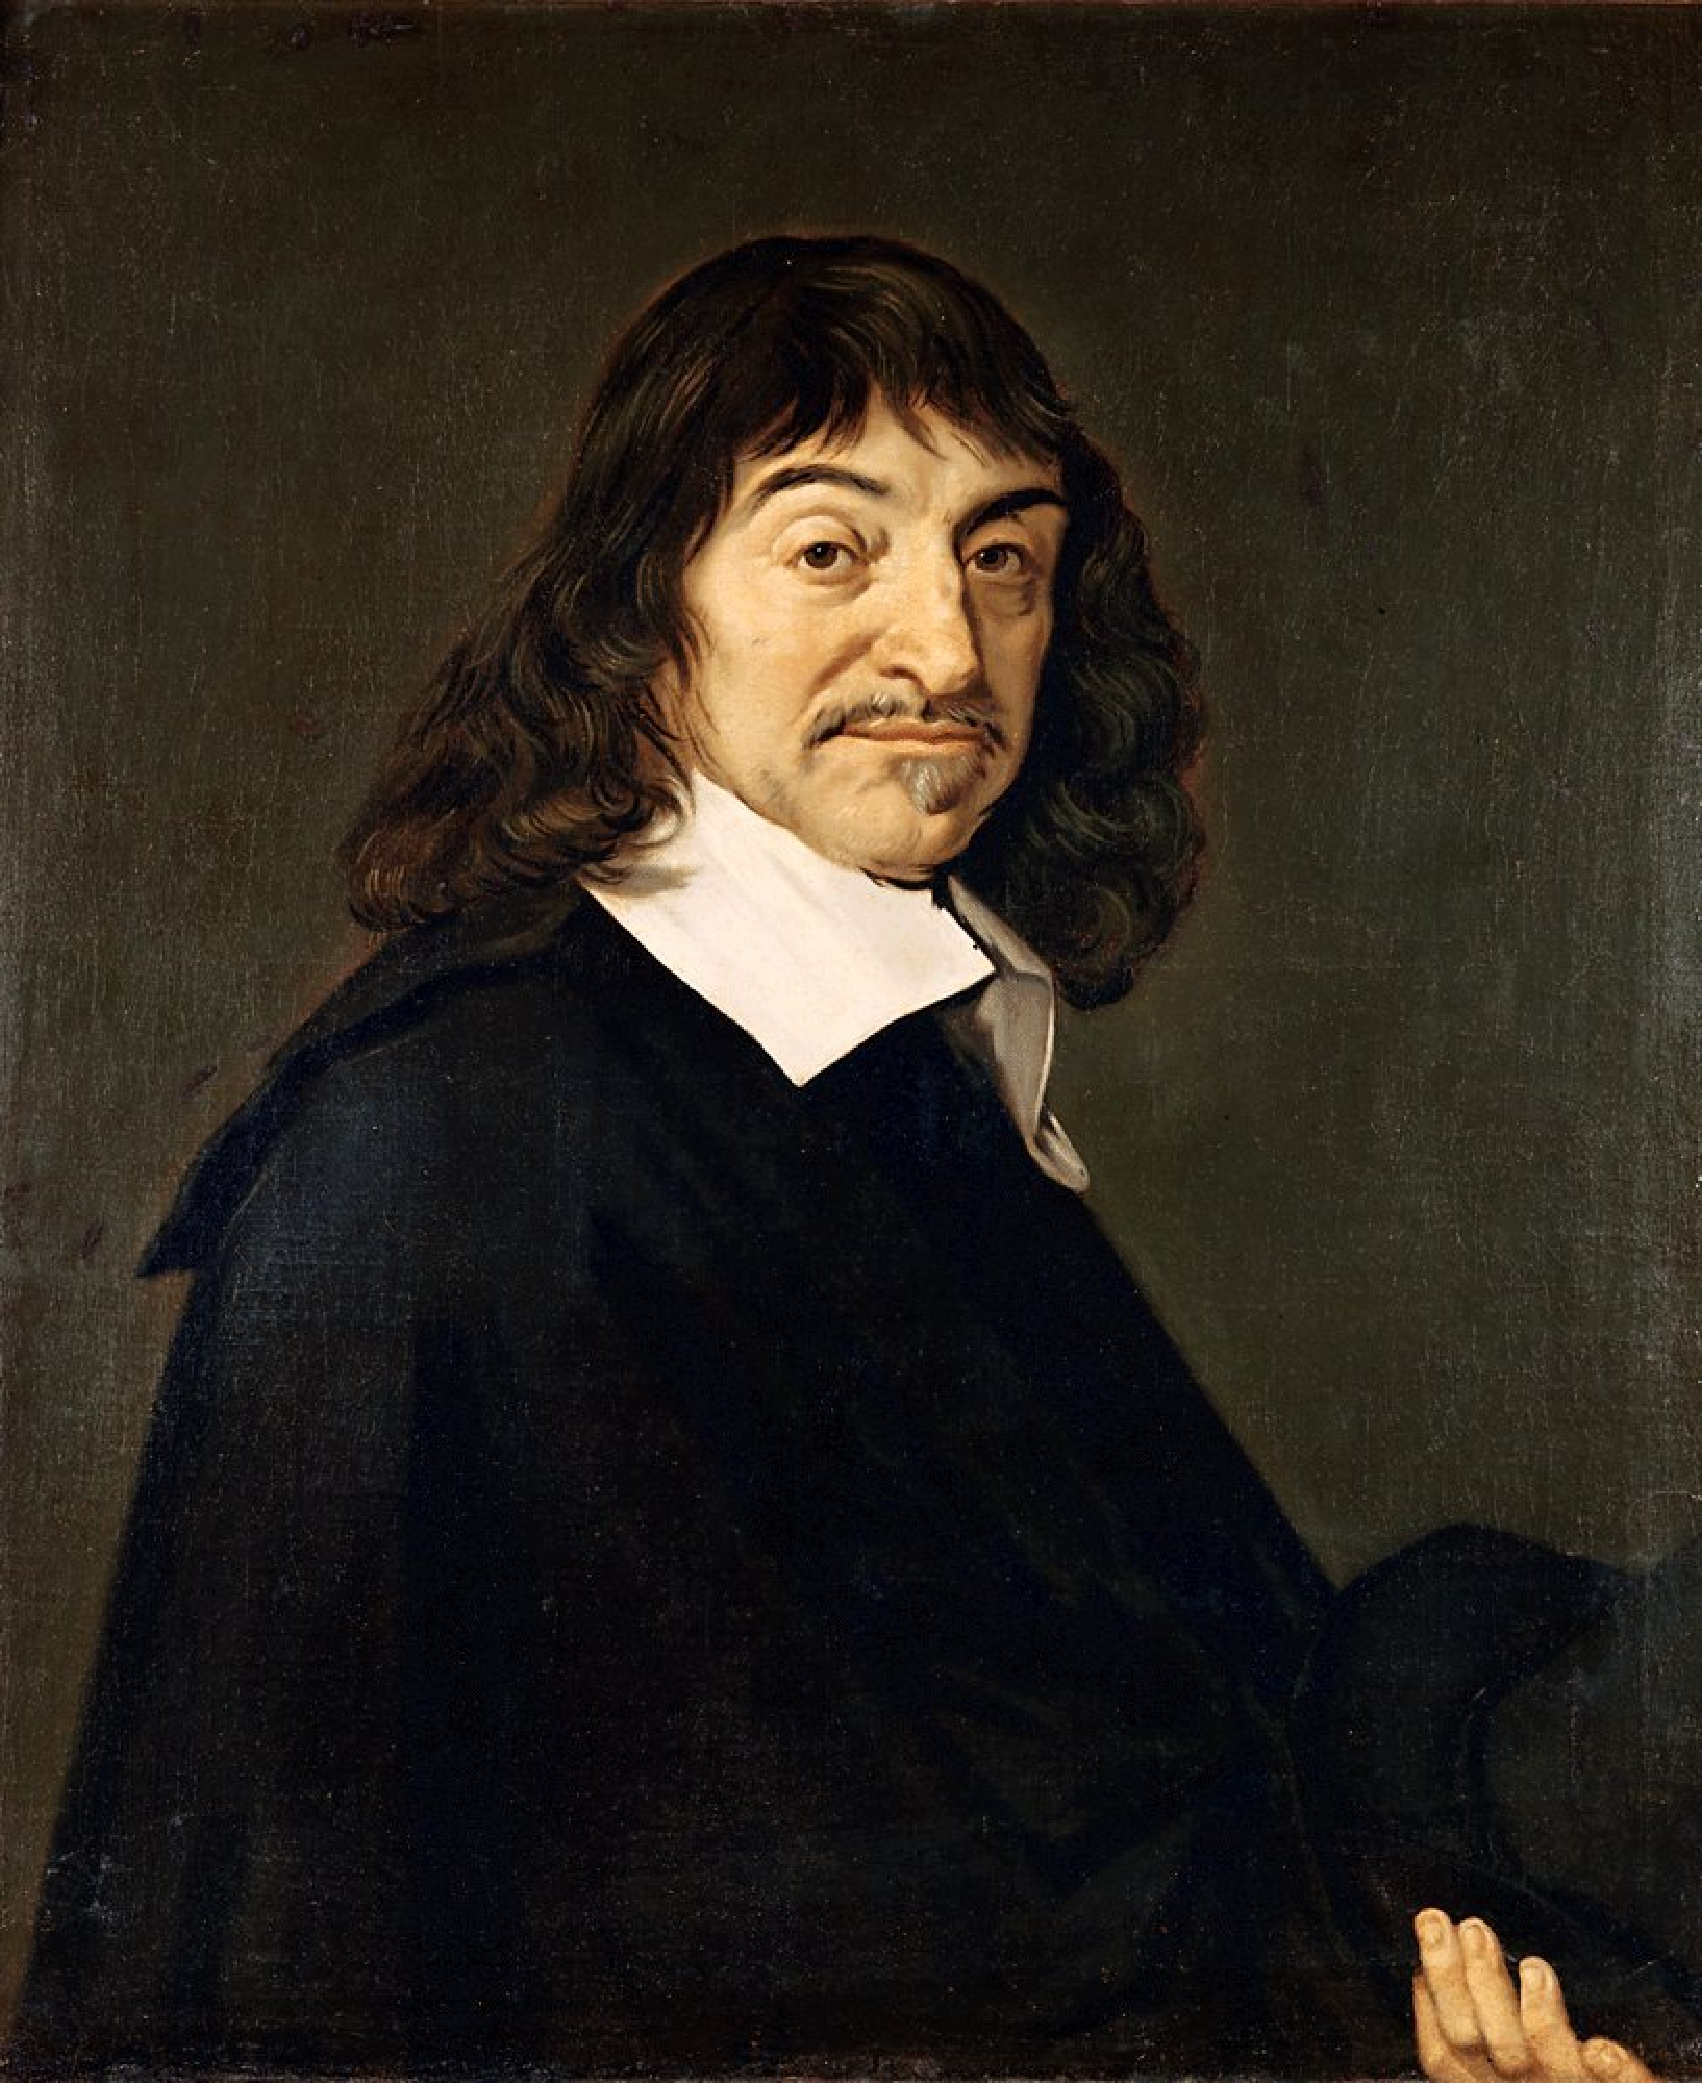
\includegraphics[scale=0.15]{Descartes.pdf}
\end{center}

\noindent
In this approach, all functions are seen as tables,
or, equivalently, as unbounded multidimensional
spreadsheets:

\paragraph{Multiplication table}
\[
\begin{array}{r@{}r|rrrrrrr}
&\multicolumn{1}{r}{} & & & & & & x & \rightarrow \\
\multicolumn{2}{@{}c|}{x\times y} & 0 & 1 & 2 & 3 & 4 & 5 & \ldots \\
\hline
& 0 & 0 & 0 & 0 & 0 & 0 & 0 & \ldots \\
& 1 & 0 & 1 & 2 & 3 & 4 & 5 & \ldots \\
& 2 & 0 & 2 & 4 & 6 & 8 & 10 & \ldots \\
& 3 & 0 & 3 & 6 & 9 & 12 & 15 & \ldots \\
& 4 & 0 & 4 & 8 & 12 & 16 & 20 & \ldots \\
y & 5 & 0 & 5 & 10 & 15 & 20 & 25 & \ldots \\
\downarrow & \vdots & \vdots & \vdots & \vdots & \vdots & \vdots & \vdots & \ddots
\end{array}
\]

\paragraph{Ackermann function}
\[
\begin{array}{rr|rrrrrrrrrrrrrr@{}}
&\multicolumn{1}{r}{} & & & & x & \rightarrow \\
& & 0 & 1 & 2 & 3 & \cdots \\
\hline
& 0 & 1 & 2 & 3 & 4 & \cdots \\
& 1 & 2 & 3 & 4 & 5 & \cdots \\
& 2 & 3 & 5 & 7 & 9 & \cdots \\
& 3 & 5 & 13 & 29 & 61 & \cdots \\
& 4 & 13 & 65533 & \cdots \\
y & 5 & 65533 & \cdots \\
\downarrow & \vdots & \ddots
\end{array}
\]

\paragraph{Sieve of Erastosthenes}
\[
\begin{array}{rr|rrrrrrrrrrrrrr@{}}
&\multicolumn{1}{r}{} & & & & & & & x & \rightarrow \\
& & 0 & 1 & 2 & 3 & 4 & 5 & 6 & \cdots \\
\hline
& 0 & 2 & 3 & 4 & 5 & 6 & 7 & 8 & \cdots \\
& 1 & 3 & 5 & 7 & 9 & 11 & 13 & 15 & \cdots \\
& 2 & 5 & 7 & 11 & 13 & 17 & 19 & 23 & \cdots \\
& 3 & 7 & 11 & 13 & 17 & 19 & 23 & 29 & \cdots \\
y & 4 & 11 & 13 & 17 & 19 & 23 & 29 & 31 & \cdots \\
\downarrow & \vdots & \vdots & \vdots & \vdots & \vdots & \vdots & \vdots & \vdots & \ddots
\end{array}
\]

With the hyperdaton, there is no need to describe the “evolution” of a
variable, either through space or time or with respect to some virtual
dimensions, since one can simply consider the Cartesian product of all
of the possible dimensions---including time and space---to create an
index and then to demand the value of that variable at that point.

\paragraph{The project.}
We successfully developed a compiler for TransLucid,
a declarative language supporting Cartesian programming.
The approach taken was to develop the hyperdaton data structure
in~C++0x (the next standard for~C++), and to create an infrastructure
in which one could write Cartesian programs in TransLucid, in~C++
or in a mix of the two.  This approach guarantees a simple Cartesian
semantics for the result, whether a declarative or imperative approach
is taken, and ensures that quality code can be generated.

The implementation takes advantage of a number of recently released
libraries, in particular \url{Boost::Spirit} for creating attribute
grammars, parsers and pretty-printers, and of many of the features of
C++0x, including variadic templates, Unicode characters and strings,
and lambda functions.  Because C++'s template mechanism allows compile-time
programming, we are capable of producing very tight and efficient code.
We also found a bug in the GNU C++0x compiler extensions for rvalue 
references, which is now fixed.

The resulting implementation will be used for a number of different
applications, including reactive programming, multidimensional hypertext
and multidimensional blogging.
\end{multicols}
\end{document}
The implementation language was~C++0x, the soon-to-be-released standard
for~C++, and we used the Gnu C++ compiler, fixing


The multidimensional nature of the hyperdaton supports a \emph{Cartesian}
approach to computing.  Descartes radically simplified geometry by giving
it an algebraic basis; the simplicity of the coordinate system that he
introduced made previously difficult problems trivial, and laid the
foundations for
all of modern mathematics and science.  Similarly,

The TransLucid programming language is a low-level intensional
language, designed to be sufficiently rich for it to be the
target language for translating the common programming paradigms
into it, while still being fully declarative.
The objects manipulated by TransLucid, called hyperdatons, are
arbitrary-dimensional infinite arrays, indexed by multidimensional
tuples of arbitrary types.


We present the syntax, denotational and operational semantics for
a simple TransLucid system, consisting of 1)~a header detailing how
expressions should be parsed, 2)~a set of libraries of types, and
operations thereon, defined in a host language, 3)~a set of TransLucid
equations, and 4)~a TransLucid demand to be evaluated.

The evaluation of a demand for an $(\textit{identifier},\textit{context})$
pair is undertaken using eduction, where previously computed pairs are
stored in a cache called a warehouse. The execution ensures that only
those dimensions actually encountered during the execution of an expression
are taken into account when caching intermediate results.

%\noindent
%\textbf{Keywords:} Cartesian programming, Lucid language,
%declarative programming, multidimensional programming,
%context-aware programming, semantics.

\section{Introduction}
\label{sec:intro}

This paper presents the TransLucid programming language, in which
variables define \emph{hyperdatons}, infinite multidimensional arrays
of arbitrary dimensionality, indexed by dynamically generated lazy tuples.
The infinite nature of the hyperdatons allows the natural encoding of
the set of possible states in an imperative language or the set
of possible functions in a functional language; it is even possible
to encode hyperdatons of functions, thereby providing a simple solution
to adding higher-order functions to the Lucid programming
language~\cite{bk:lucid}.
The lazy tuples---reminiscent of those of Linda~\cite{linda}---and
the declarative nature of the language ensure that
an easily written, efficient, multithreaded implementation can be generated.

The original version of TransLucid used eager tuples and was presented
in~\cite{phd:ditu}---we now call that language Eager TransLucid.  The
history of the development leading from the original Lucid to TransLucid
is presented in~\cite{art:histLucid}.  The eductive implementation of Eager
TransLucid
is given in~\cite{art:eagerTL}.  The first multithreaded implementation
of TransLucid is given in~\cite{art:multithreadedTL}.
The TransLucid language is now being developed into a production language,
allowing the use of user-defined atomic data types and operations. 

The main contribution of this article is to further develop the eductive
implementation of TransLucid, which caches intermediate results, ensuring
that only dimensions of relevance are stored in the cache.  The solution
offered here ensures that this minimality is preserved when additional
variables are introduced and when lazy tuples are used.  Furthermore,
the given rules can be transformed into a variety of physical architectures. 

This article begins by presenting a small TransLucid
example~(\S\ref{sec:example}).  We continue with the
presentation of the syntax for a simple TransLucid
system~(\S\ref{sec:system}), consisting of a header,
libraries, equations and a demand.  The denotational
semantics~(\S\ref{sec:semantics}) defines the domains manipulated
by TransLucid and defines how demands are interpreted.  The operational
semantics~(\S\ref{sec:operational}) forms the core of the paper.
The conclusions~(\S\ref{sec:conclusions}) discuss future work.
